\documentclass[11pt,a4paper]{article}
\usepackage[left=2.3cm,top=2cm,right=2.3cm,nofoot]{geometry}
\usepackage{geometry}
\usepackage{amsmath}
\usepackage{amssymb}
\usepackage{txfonts}
\usepackage{microtype}
\usepackage{epsfig}
\usepackage{graphicx}
\usepackage{moreverb}
\usepackage{hyperref}
\usepackage{listings}
\usepackage{xcolor}
\usepackage{textcomp}
\usepackage{makecell}
\usepackage{wasysym}
\definecolor{listinggray}{gray}{0.98}
\definecolor{lbcolor}{rgb}{0.98,0.98,0.98}
\lstset{
	backgroundcolor=\color{lbcolor},
	tabsize=4,
	rulecolor=,
	language=matlab,
    basicstyle=\scriptsize\ttfamily,
    upquote=true,
    aboveskip={1.5\baselineskip},
    columns=fixed,
    showstringspaces=false,
    extendedchars=true,
    breaklines=true,
    prebreak = \raisebox{0ex}[0ex][0ex]{\ensuremath{\hookleftarrow}},
    frame=single,
    showtabs=false,
    showspaces=false,
    showstringspaces=false,
    identifierstyle=\ttfamily,
    keywordstyle=\color[rgb]{0,0,1},
    commentstyle=\color[rgb]{0.133,0.545,0.133},
    stringstyle=\color[rgb]{0.627,0.126,0.941},
}

\usepackage{tikz}
\usepackage{pgfplots} 
\usepackage{pgfgantt}
\usepackage{pdflscape}
\usepackage{subcaption}
\usepackage{adjustbox}
\usepackage{siunitx}
\pgfplotsset{compat=newest} 
\pgfplotsset{plot coordinates/math parser=false}
\usepackage{pdfpages}
\usepackage{placeins}
\usepackage{wrapfig}





\newlength\fwidth
\newlength\fheight
\pagestyle{myheadings}

\pgfplotsset{every axis/.append style={
        scaled y ticks = false, 
        scaled x ticks = false, 
        y tick label style={/pgf/number format/.cd, fixed, fixed zerofill,
                            int detect,1000 sep={\;},precision=3},
        x tick label style={/pgf/number format/.cd, fixed, fixed zerofill,
                            int detect, 1000 sep={},precision=3}
    }
}

\usepackage{eso-pic}
\usepackage{ifthen}

\usepackage[nottoc]{tocbibind}
\usepackage[backend=biber,style=numeric,sorting=none]{biblatex}
\addbibresource{bibben.bib}

\usepackage{float}
\usepackage{subcaption}
\usepackage{gensymb}
\usepackage{siunitx}
\usepackage{enumitem}

\title{Project 2b: Bayesian Optimization}
\author{
  Kevin Andersson\\
  \texttt{kevinan@student.chalmers.se}
  \and
   Eric Lindgren\\
  \texttt{ericlin@chalmers.se}
}

\markright{Kevin Andersson and Eric Lindgren, Group 7}

\begin{document}

\maketitle

\pagenumbering{gobble}% Remove page numbers (and reset to 1)
% \newpage
\pagenumbering{arabic}% Arabic page numbers (and reset to 1)
\setcounter{page}{1}
\section{Introduction and Background}

One system of interest in materials science is one where an adsorbed atom, an adatom, is located on top of a crystal surface \cite{wiki_adatom}. The position of the adatom on the surface affects the total potential energy of the system, and thus the position of the adatom $(x,y)$ parametrizes a potential energy surface (PES) $E(x,y)$ for the system. However, there are two main problems when simulating such a system. First, finding the position of the adatom that results in the lowest energy is difficult since the PES often has multiple local minima \cite{project_pm}. Secondly, the system potential energy is often obtained using Density Functional Theory (DFT), and hence it may be computaionally intractable to perform many evaluations of the potential energy.

Both of these challenges will be tackled in this report using Gaussian Processes (GP). The first problem will be approached using Bayesian Optimization, and for the second problem we will train a general purpose model for the PES using only $\sim 100$ potential energy samples. This general purpose model can then be used instead of DFT to study various properties of the adatom \cite{project_pm}. We will specifically apply the general purpose model to predict the potential energy along a transition path for the adatom between two points on the crystal surface, and compare this to the ground-truth transition path as obtained from the PES.

The system of interest in this report is an Au-surface with an Au adatom. Note that this system will be simulated using atomistic simulations through the Python package \texttt{ASE} \cite{ASE}, and specifically that the ground-truth PES is being computed through Embedded Medium Theory (EMT) calculations rather than DFT \cite{project_pm}. However, this report still exemplifies the usefulness of Bayesian Optimization and GP-models for functions that are difficult to evaluate.

\section{Methodology}

In this section we present our methodology for analyzing and approximating the potential energy surface (PES) using Bayesian optimization for a Au surface with an Au atom placed on top. But before we go into detail on the Bayesian optimization, we first present the ground-truth PES that will be used as a basis for the optimization, as well as the results for trying to find the global minimum of the PES using naive local search.


\begin{figure}[ht]
    \centering
    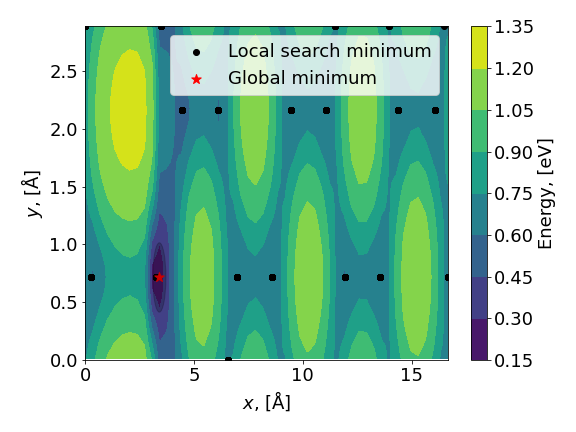
\includegraphics[width=0.7\textwidth]{figures/task12.png}
    \caption{Obtained potential energy surface (PES) together with the global minimum (red star) and the minima as obtained through a naive local search with 500 individual walkers (black dots). }
    \label{fig:pes}
\end{figure}

The Au system was simulated using \texttt{ASE}, a Python package for atomistic simulations \cite{ASE}, with the surface being given. In order to obtain the PES $E(x,y)$, the surface atom was introduced at different coordinates $(x,y,z)$ with $z$ being set so that the surface atom was placed some distance above the surface, after which the system was relaxed using BFGS as implemented in \texttt{ASE}. Since the PES is periodic, we only study the primitive cell $x\in\left(0,16.65653\right)$, $y\in\left(0,2.884996\right)$. The $(x,y)$ values formed a 50x50 grid, and the obtained PES is given in figure \ref{fig:pes}, with the global minimum being marked with a red star with coordinates $(3.4, 0.71)$. Note that there are many local minima in the PES; a quick visual inspection yields that there are at least 12 local minima. We thus expect that conducting a local search to find the global minimum starting from random positions $(x,y)$ should succeed with a probability around $p \approx 1/12 \approx 8\%$. We performed such a search using 500 walkers with random starting positions, which were then minimized using the \texttt{minimize} function from the Python package \texttt{Scipy}, which was setup to use the gradient-based L-BFGS-B method \cite{scipy_min}. The optimum found by each walker are given in figure \ref{fig:pes} as black dots. The local search resulted in 11.6\% of the walkers converging to the global minimum, which is slightly higher than our expectation, but still highlights the difficulty of performing optimization in complex energy landscapes using (naive) local gradient descent-based algorithms. Thus it is motivated to use methods such as Bayesian optimization, which we will focus on throughout the rest of this report. 


\subsection[Task 1]{Task 3: Bayesian Optimization}
\label{sec:method_task3}
In this task we applied a Bayesian optimization algorithm to find the global minimum, while sampling the PES as few times as possible. In general, sampling the PES or any other multidimensional function can be very expensive and time consuming. The Bayesian optimization algorithm is based on Gaussian processes (GP), which can be viewed as an infinite dimensional Gaussian distribution where each point in the $(x,y)$-plane is a dimension. The function modelled by the GP (the PES) is then uniquely determined via the GPs covariance function. So by conditioning the GP on some data, we obtained a distribution for the PES everywhere in the $(x,y)$-plane. In this task we used the GPy package to handle the implementation of the GP so we only needed to choose how to determine the covariance function. The covariance function was modelled by a kernel and we used the radial basis function (RBF) kernel which looks like 
\begin{equation*}
    k(x, x') = \sigma^2 \text{exp}(-\frac{1}{2l^2}||x - x'||_{L2}^2),
\end{equation*}
where $\sigma^2$ and $l$ are two parameters known as the kernel variance and the kernel length scale. The kernel variance is in a way the amplitude of the covariance and thus describes how large the variations are in the PES. From figure \ref{fig:pes} we see that the PES has minimum and maximum at 0.2 eV and 1.3 eV, so the standard deviation is around 0.3 and the variance is then around 0.09. Based on this we set a gamma distributed prior for $\sigma^2 \sim \mathcal{G}(1,0.1)$. The length scale determines how far apart the points are regarded as correlated, or in other words over how large regions the PES is roughly constant or slowly varying. From figure \ref{fig:pes} we observe that the PES is roughly constant over distances $\sim \SI{0.5}{Å}$. We thus set a prior for the length scale to be a gamma distribution $\mathcal{G}(2,0.5)$. Furthermore we also added a bias kernel to increase the performance of our GP.


We have now described the basics of a GP and specified a kernel with priors for our parameters. We can thus, by training the GP on some initial data, make a prediction $\mu(x,y)$ with standard deviation uncertainty $\delta(x,y)$ over the whole primitive cell. To search for the global minimum we want to sample a new point, and we thus need to define where to sample this new point, based on our prediction. We define the acquisition function
\begin{equation}
    \label{eq:acquisition_function}
    A(x,y) = -\mu(x,y) + \beta \delta(x,y),
\end{equation}
where beta is a hyper parameter we must choose. By finding the point where the acquisition function has a maximum we sample points where the PES is low and where the GP is uncertain, and the hyper parameter thus balances between exploitation or exploration in the algorithm. The implementation of the algorithm consisted of the following steps. First, evaluate the PES at 5 random points, train the GP model using these points and then do a prediction of the PES. From the prediction, evaluate the PES again for the point obtained by maximizing the acquisition function, and then train a new GP with the new data point added to the old data points. This is then repeated until one is satisfied with the sampling.  

So we now have the complete Bayesian optimisation algorithm and the next part is to decide a good value of the hyper parameter $\beta$. To do this we performed the optimization for many values of $\beta \in (1,5)$ and then evaluated the performance by studying the convergence. So keeping in mind that we generally want to find the global minimum and evaluate the PES as few times as possible we define convergence to be when the GP finds the global minimum. With this definition we can decide the hyper parameter by choosing the $\beta$ that resulted in the least amount of samples. 





















\subsection[Task 4]{Task 4: Transition path barriers}
\label{sec:method_task4}

In this task, we study GPs as a way of emulating the full PES. Using GPs to emulate the PES yields a fast model which can be used to compute various properties related to the adatom \cite{project_pm}. In this case, we will specifically focus on using the GP model to analyze a transitional path barrier. 

Here we will study the specific transition path through the PES that connects the point $(11,2.1)$ with the global minimum at $(3.4,0.71)$. An arbitrary path between the points $(x_1,y_1)$ and $(x_2,y_2)$ can be parameterized by a parameter $\lambda$ that varies between $0\rightarrow1$ as

\begin{equation}
    (x,y) = \left(x_1, y_1 \right ) + \lambda \left(x_2-x_1, y_2-y_1 \right).
\end{equation}
Thus by evaluating the GP mean of the obtained model for points $(x,y)$ for various $\lambda$, we could obtain a transition path as a function of $\lambda$. In our specific case, the starting point $(x_1,y_1)$ was the global minimum and the end point $(x_2,y_2)$ was the point $(11,2.1)$. The uncertainty in the GP prediction along the path was estimated by evaluating the GP variance along the same points $(x,y)$. These results could then be compared to the Bayesian Optimization GP with optimal $\beta$ from Task 3, where the model was trained until convergence was reached, and the ground-truth PES evaluated along the same path. 

In order to obtain a general-purpose GP model that emulates the ground-truth PES to a high degree, we require a slightly different sampling behaviour as compared to the previous task in section \ref{sec:method_task3}. The key quantity to minimize is the overall uncertainty of the GP over the $\{x,y\}$-domain, and hence we want to sample points where the GP uncertainty is the largest. Thus, the acquisition function in equation \eqref{eq:acquisition_function} was modified by letting $\beta \rightarrow \infty$ \cite{project_pm}. The GP model was then trained by sampling points according to this modified acquisition function, and the convergence of the model was monitored by computing the RMSE (root-mean-squared-error) of the GP mean as compared to the ground truth PES. The same priors and number of initial data points as in task 3, section \ref{sec:method_task3}, where used.








\section{Results and discussion}

In this section we present our result for Bayesian optimization of the PES, as well as for the practical application of studying a transition path for the adatom on the Au-surface.

\subsection[Task 1]{Task 3: Bayesian Optimization}
\label{sec:results_task3}
To study the model for different values of the hyper parameter $\beta$ figure \ref{fig:task3_iter} is presented. The figure describes how many iterations the optimization algorithm required before it found the global minimum. From the figure it is clear that the algorithm does not converge for all values of beta. In particular for small $\beta$ the algorithm never finds the global minimum within the number of cutoff iterations. However, observe from the figure that large $\beta$ demands more iterations before convergence. Both of these features seems reasonable; for small $\beta$ the algorithm is more likely to keep sampling a local minimum instead of exploring more of the space. This results in a sensitivity for the location of the starting point and we end up in the same situation we got for the naive search on task 2. For large $\beta$ we are on the other hand more inclined to explore new parts of the space even if we already have samples near the global minimum. Thus, for large $\beta$ the algorithm becomes very dependent on the convergence condition; how close to the global minimum do you need to sample to say you have found it? So from the figure we seem to have a optimal value for the hyper parameter somewhere around $\beta = 2.6$, for which the algorithm finds the global minimum in the fewest number of iterations. However this result is only valid for when we send in this particular set of initial data. For another set of data which is closer to the global minimum the algorithms with low $\beta$ might find it much faster. But also if the global minimum would have been further away from the initial data maybe algorithms with $\beta$ equal or higher then the observed optimal $\beta$ also would have had trouble finding it. So to decrease this uncertainty and be more confident in the choice of beta one should do this sweep over the hyper parameter many times where different initial data is used and then present the average number of iterations.

To further extend on this analysis, the choice of convergence criteria is a bit arbitrary and can highlight different aspects of the algorithm. An alternative definition of convergence could for example be when the algorithms samples the same point (to some tolerance) two or more times in a row. This convergence criterion is probably also very sensitive to the initial data, but if that uncertainty is eliminated (as described above) algorithms with lower $\beta$ should always converge faster. The problem is that it does not always converge to the global minimum so one here also needs to consider how many times (different initial data) the algorithms finds the global minimum for each value of $\beta$, and then find the $\beta$ that balances the convergence and efficiency of finding the global minimum. To use this convergence condition may be more reasonable since we in a general situation do not know the global minimum and then needs some other condition on when to stop sampling. On the other hand, the thing we really are interested in is to find the global minimum with as few evaluations of the PES as possible which the convergence condition we used highlights. However both of these convergence conditions to decide $\beta$, especially the condition we used, probably generalize poorly to other functions since it could be very sensitive to the specific form of the function.

\begin{figure}[ht]
    \centering
    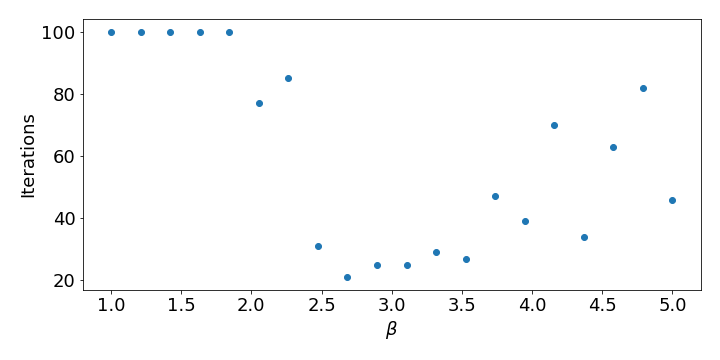
\includegraphics[width = 0.6\textwidth]{figures/task3_iter.png}
    \caption{Number of iterations required for the algorithm to find the global minimum for different values of the hyper paramer $\beta$.}
    \label{fig:task3_iter}
\end{figure}

Once we had decided on a good value for $\beta = 2.6$ we reran the algorithm and the result is presented in figure \ref{fig:task3_pred}. In the figure we see the prediction of the GP for the PES together with the predicted uncertainty and the acquisition function. These are for the last step in the algorithm, i.e when the model had converged. From the mean plot we can clearly see that the model has found the global minimum and captures the features of the PES close to the minimum. For other regions however the GP does not capture the PES, which is good since we only are interested in finding the global minimum. From the figure we also see a heat map for the standard deviation uncertainty over the primitive cell. We can see that the uncertainty varies a bit over the cell and is generally much lower near the samples, which is expected. We also notice that the uncertainty seems to be largest around the maximas of the PES seen in \ref{fig:pes}. This is also very reasonable since maxima are the least interesting to sample according to the acquisition function. Finally, in the figure we also see the acquisition function which as expected balances the search of the found minimum and the uncertain areas.


One interesting observation that can be made from the figure is that many of the sampled points lay along the edges of the primitive cell. This feature was generally observed when performing the optimization and was even more prominent when we had more samples. We conclude that this must be because the GP becomes much more uncertain in its prediction near the edges. This is reasonable since the edge breaks the symmetry of where nearby sampled points are located, from which we can use in the inference. This effectively leads to the GP almost performing some sort of extrapolation instead of an interpolation near the edge. However, we know that the primitive cell is periodic so in a sense we have sampled points outside the boundary. This knowledge of the periodicity is unfortunately not used in the GP. Having said that, this can be built into the GP by using a periodic kernel instead. We made some attempts with the Standard periodic kernel but had some trouble with instability of the method. But when it worked the sampling was distributed much better over the primitive cell and we avoided sampling the edge over and over again. Ultimately this leads to the need for fewer samples and we strongly believe that the best way to sample this PES is to use the knowledge of periodicity in the GP by encoding it in the kernel. 


\begin{figure}[ht]
    \hspace{-50pt}
    %\centering
    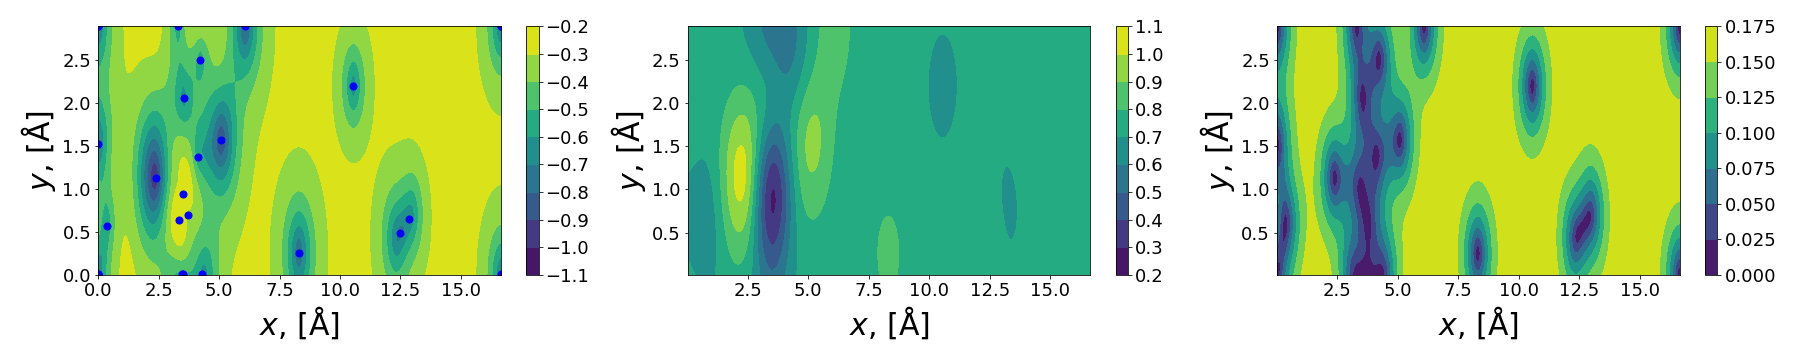
\includegraphics[width = 1.2\textwidth]{figures/task3_pred.png}
    \caption{To the left the acquisition function when the the algorithm find the global minimum together with the initial and sampled data points. In the middle the mean prediction of the GP over the PES and to the right the GPs uncertainty in its prediction. }
    \label{fig:task3_pred}
\end{figure}

\subsection[Task 4]{Task 4: Transition path barriers}
\label{sec:results_task4}

We finally turn to the results for the use of a general-purpose GP as a proxy for the PES, and how it can be used to predict a transition path for the adatom on the Au surface. The RMSE as monitored during training of the GP is given in figure \ref{fig:task4_rmse}. The RMSE is computed as the root-mean-squared error between the GP mean and the ground-truth PES, and is given as a function of the number of training samples as acquired by the modified acquisition function. We note that the training RMSE features some plateaus. The plateaus could correspond to local minimum in the GP optimization landscape, or that some of the sampled points do not contain enough information to improve the GP mean prediction. We observed during training that a substantial number of samples where drawn from the boundary of the primitive cell. As discussed in Task 3, the symmetry break induced by the edge may lead to an artificially high uncertainty, which means that these points will be sampled without contributing all that much to the mean prediction. However, after around 120 samples the RMSE starts to decrease monotonously, and seems to flatten out at around 150 samples at a low training RMSE of $\SI{0.04}{eV}$. We thus conclude that around 150 samples are required to reach a general GP that represents the ground-truth PES well. This is fewer than what was used to computed the ground-truth PES in figure \ref{fig:pes}, where 2500 (50x50) energy samples were used, which could be an enormous difference in the cases where the PES is computationally difficult to compute.

\begin{figure}[ht]
    \centering
    \begin{subfigure}{.46\textwidth}
          \centering
          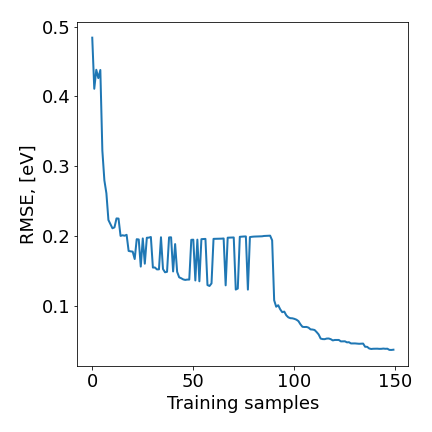
\includegraphics[width=1\textwidth]{figures/task4_train.png}
          \caption{Training RMSE for general GP}
          \label{fig:task4_rmse}
    \end{subfigure}%
    \begin{subfigure}{.46\textwidth}
          \centering
          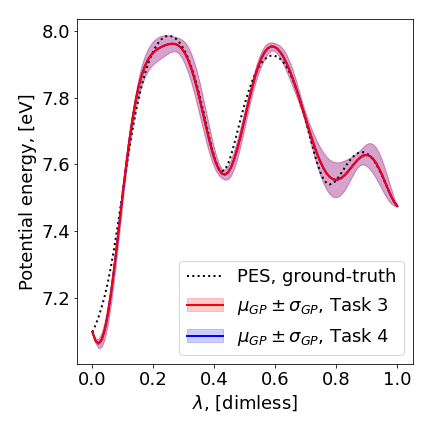
\includegraphics[width=1\textwidth]{figures/task4_path.png}
          \caption{Predicted and ground-truth transition path}
    \label{fig:task4_transition}
    \end{subfigure}
    \caption{RMSE compared to the ground-truth PES as monitored during the training of the general-purpose GP, as well as predicted and ground-truth potential energy along the studied transition path.}
    \label{fig:task4}
\end{figure}

The potential energy transition path for the adatom transitioning between the two points on the Au-surface is given in figure \ref{fig:task4_transition}. The mean predicted path from the general GP (referred to as Task 4), $\mu_{GP}$ is given as the blue filled line, with a one standard deviation error band obtained from the GP variance, $\sqrt{\sigma^2_{GP}}$, represented by the blue shadowed area. The mean predicted path for the Bayesian optimization GP (Task 3) is given as the red dashed line, with the one standard deviation error band given by the red shadowed area. Finally, the ground-truth transition path as obtained from the PES is given as the dotted black line. We observe that the general purpose GP follows the ground-truth PES fairly well with it being mostly covered by the one-standard deviation error band, whilst the Bayesian optimization GP only manages to capture some of the rough features of the PES. Furthermore, the general-purpose GP model deviates from the ground-truth around the peak at $\lambda\approx0.6$ as well as close to the global minimum, i.e. for $\lambda\approx 0$, except for at the minimum point $\lambda = 0$. The general-purpose GP variance is also generally the largest at the peaks of the PES, with it being the largest in the vicinity of the peak at $\lambda\approx0.6$. Note that the variance is larger in general for the Bayesian optimization GP than for the general-purpose GP, which can be explained by the Bayesian optimization GP being trained on $\sim20$ data points, whilst the general-purpose GP was trained on $\sim 150$ data points.

These results indicates two things. First, that the use of a general-purpose GP performs much better than one obtained by using Bayesian optimization. Perhaps unsurprisingly, this can be explained by that the two models are used to answer different questions; the Bayesian optimization algorithm aims to find the global minimum as quickly as possible (i.e. using as little data as possible), whilst the general-purpose model tries to model the ground-truth PES as closely as possible. Interestingly, the root of these different behaviours for the two models lies in the acquisition function, and highlights that the general-purpose GP is a special case of the Bayesian optimization algorithm in which exploration of the PES is the only thing that is valued ($\beta \rightarrow\infty$). Secondly, that the general-purpose GP model reproduce the PES fairly well motivates that Gaussian processes in general could be effectively used as a proxy model for the PES to compute properties of the system with reasonable accuracy, in situations where the ground-truth PES is difficult to sample and one thus has access to a limited number of data points. However, there are some deviations for the GP models, especially around the peaks and close to the global minimum ($\lambda\approx 0$) of the PES, and hence the specific GP models studied in this report may not be perfectly suitable for applications which depend on an accurate modelling in these regions. Note though that we observed during training that a lot of the sampled points for the general-purpose model ended up on the boundary of the primitive cell. It is thus possible that the use of other kernels which utilize more information of the system, such as the Standard periodic kernel discussed in Task 3, may lead to a better sampling of the primitive cell, and by extension to a better representation of the PES in the regions where the general-purpose GP deviates from the ground-truth.

% TODO Lägg till modell från task 3

\printbibliography

\end{document}
